\documentclass[conference]{IEEEtran}
\usepackage[utf8]{inputenc}
\usepackage{amsmath,amssymb}
\usepackage{graphicx}
\usepackage{booktabs}
\usepackage{siunitx}
\usepackage{xcolor}
\usepackage{url}
\usepackage[hidelinks]{hyperref}
\graphicspath{{figs/}}

% Remaining TODO markers are deliberate: search for TODO before submission.
\newcommand{\todo}[1]{\textcolor{red}{[TODO: #1]}}

\begin{document}

\title{Where Does the Block Parallelism Go?\\
Characterising Connected-Component Decomposition of the Graphical Lasso
on Multicore CPUs and a Consumer GPU}

\author{
\IEEEauthorblockN{Abhyuday Gandhi, Shreyas S Hegde, Shrikrishna Bhakhta}
\IEEEauthorblockA{\todo{Department, Institution, City, Country}\\
\todo{emails}}
}

\maketitle

\begin{abstract}
The graphical lasso decomposes exactly into independent subproblems, one per
connected component of the thresholded sample covariance. This looks like a
natural source of parallelism. We characterise how much of it is usable in
practice: on a multicore CPU and on a consumer laptop GPU, across four
block-size regimes, three sample sizes and problem dimensions up to $p=3200$,
with every result tied to a recorded code version and machine state.
We find that (i) decomposition yields a median $2.3$--$2.6\times$ speedup
(across three independent instances, excluding four cells whose optimal
regularisation lies below our grid) against an 8-thread CPU baseline at the
statistically best regularisation, and the
multithreaded baseline erodes the gain as $p$ grows; (ii) speedup and
estimation quality pull in opposite directions, so the fastest
regularisation is never the useful one;
(iii) the runtime is dominated by per-block interpreter overhead, not by the
eigendecompositions a cubic cost model predicts; and (iv) the true blocks are
fused by the estimator itself, not by the screening step: screening is exact,
and a few percent of spurious cross-block entries suffice to merge all true
blocks into one component. Batching the per-block work gives
$1.2$--$1.7\times$ on the CPU. On a consumer GPU in double precision, the
batched solver overtakes the CPU only when one block of $\approx1950$
variables dominates. A precision diagnostic with pre-registered accuracy
criteria shows why: in single precision the crossover falls to
$\approx650$ variables, but GPU single precision fails to converge on small
blocks, so we keep double precision as the reference result.
\end{abstract}

\begin{IEEEkeywords}
graphical lasso, sparse inverse covariance, parallel computing, GPU,
batched linear algebra, mixed precision, reproducibility
\end{IEEEkeywords}

% =====================================================================
\section{Introduction}

Sparse inverse covariance estimation with the graphical lasso
\cite{friedman2008,banerjee2008} is a standard tool for learning conditional
independence structure. Its cost is dominated by $O(p^3)$
eigendecompositions per iteration, which limits it at large $p$.
A classic result makes the problem embarrassingly parallel in principle:
the connected components of the thresholded sample covariance
$\{(i,j): |S_{ij}|>\lambda\}$ are exactly the connected components of the
graphical lasso solution, so each component can be solved independently
\cite{witten2011,mazumder2012}. The GGLasso package \cite{gglasso2021} exposes
this as \texttt{block\_SGL}.

It is tempting to conclude that more components mean more parallel speedup,
and that a GPU, which excels at many independent small problems, is the
natural accelerator. This paper tests both conclusions through three
research questions:
\begin{description}
\item[RQ1] How much does component decomposition speed up the graphical lasso
  at a statistically useful regularisation, against a fair multithreaded CPU
  baseline, and why is the gain not larger?
\item[RQ2] Does batched execution of the per-block work help, on a CPU and on
  a consumer GPU, and what limits it?
\item[RQ3] Is GPU memory a binding constraint at the problem sizes where a GPU
  could help?
\end{description}

\textbf{Contributions.}
\begin{itemize}
\item A controlled characterisation of component decomposition across
  384 configurations per thread setting, reporting speedup only at the
  statistically best regularisation, with paired 1- and 8-thread runs.
\item A profiling result: the decomposed solver is bound by per-block
  interpreter overhead and dispatch, not by the largest eigendecomposition,
  so the cubic work model mispredicts wall-clock time.
\item An explanation of why little parallelism survives at useful
  regularisation: screening is exact, and the \emph{estimator} fuses the true
  blocks through a small number of spurious cross-block entries.
\item A batched ADMM solver (NumPy and PyTorch backends) and a measurement of
  where a consumer GPU helps, separating the effect of batching from the
  effect of floating-point precision, with pre-registered accuracy criteria.
\item A reproducibility account: two subtle environmental faults that
  invalidated earlier datasets, and the provenance tooling that caught them.
\end{itemize}

% =====================================================================
\section{Related Work}
\textbf{Graphical lasso solvers.} The graphical lasso \cite{friedman2008,
banerjee2008} has been solved by block coordinate descent \cite{friedman2008},
alternating linearisation \cite{scheinberg2010}, ADMM \cite{boyd2011}, and
second-order methods such as QUIC \cite{hsieh2014quic}, whose BigQUIC variant
solves problems with a million variables on a single machine using
block-coordinate descent over clustered blocks and bounded memory
\cite{hsieh2013bigquic}. Mazumder and Hastie \cite{mazumder2012ejs}
analyse the convergence behaviour of the block coordinate algorithm. We do not
propose a new solver; we study how much parallelism the exact component
decomposition exposes to an existing ADMM solver \cite{gglasso2021}.

\textbf{Screening.} Witten et al.\ \cite{witten2011} and Mazumder and Hastie
\cite{mazumder2012} showed that thresholding the sample covariance yields the
exact component structure of the graphical lasso solution, and used it to
solve large problems block by block. Fattahi and Sojoudi \cite{fattahi2019}
give conditions under which thresholding reproduces the solution's entire
sparsity pattern. These results relate the thresholded covariance to the
graphical lasso \emph{estimate}; they say nothing about how the estimate's
components relate to the planted block structure. That second relation is
what decides how much block parallelism is usable, and it is what we
measure: screening is exact on our instances, yet the estimate fuses the true
blocks at statistically useful regularisation.

\textbf{Batched and GPU linear algebra.} Batched BLAS and LAPACK interfaces
target many small independent matrix problems, where per-call launch overhead
dominates arithmetic \cite{dongarra2017batched}. Our batched ADMM follows
this design, and our measurements show the same overhead-bound behaviour for
small blocks on both CPU and GPU.

\textbf{Mixed precision.} Lower precision can accelerate numerical linear
algebra substantially on GPUs, but requires care about accuracy and
convergence \cite{higham2022mixed,abdelfattah2021survey}. We evaluate single
precision against acceptance criteria fixed before measurement, and find it
accurate on large blocks but non-convergent on small ones on the GPU.

\textbf{Benchmarking methodology.} Hoefler and Belli \cite{hoefler2015}
catalogue common pitfalls in reporting parallel performance. Our
reproducibility section adds two concrete, silent failure modes: random data
that depend on the BLAS thread count, and an uncontrolled machine state that
biased CPU-versus-GPU comparisons.

% =====================================================================
\section{Background}

\subsection{Graphical lasso and ADMM}
Given a sample covariance $S\in\mathbb{R}^{p\times p}$, GGLasso solves
\begin{equation}
\min_{\Theta\succ 0}\; -\log\det\Theta + \operatorname{tr}(S\Theta)
 + \lambda\,\lVert\Theta\rVert_{1,\mathrm{od}},
\label{eq:glasso}
\end{equation}
with the $\ell_1$ penalty on off-diagonal entries only. Its ADMM solver
\cite{boyd2011} alternates an eigendecomposition-based update of $\Omega$,
an off-diagonal soft-threshold for $\Theta$, and a dual update, with
adaptive penalty $\rho$ and Boyd's primal/dual residual stopping test.
Every iteration costs one $p\times p$ symmetric eigendecomposition.

\subsection{Exact screening}
Witten et al.\ \cite{witten2011} and Mazumder and Hastie \cite{mazumder2012}
showed that the vertex partition induced by the connected components of the
graph $\{|S_{ij}|>\lambda\}$ equals the partition of the solution of
\eqref{eq:glasso}. The problem therefore splits into independent blocks of
sizes $s_1,\dots,s_K$, and the eigendecomposition cost falls from $p^3$ to
$\sum_k s_k^3$. We call $F_{\max}=s_{\max}^3/\sum_k s_k^3$ the share of cubic
work in the largest block; it bounds the benefit of solving blocks in
parallel.

% =====================================================================
\section{Methodology}

\subsection{Synthetic ground truth}
GGLasso's generator only produces equal-sized blocks, so we assemble a
block-diagonal precision matrix from independently generated power-law
network blocks \cite{gglasso2021}. Four regimes fix the block-size
distribution: \emph{balanced} (5 equal blocks), \emph{imbalanced}
($90/4/4/1/1\%$ of $p$), \emph{many\_tiny} (blocks of $\approx 20$), and
\emph{one\_giant} (a single block). We draw $n$ samples from
$\mathcal{N}(0,\Theta^{-1})$ using a Cholesky factor; Section~\ref{sec:repro}
explains why the sampling method matters.

\subsection{Experimental grid}
RQ1 sweeps $p\in\{100,200,400,800\}$, $n/p\in\{2,5,10\}$ and
$\lambda\in\{0.05,0.10,\dots,0.40\}$ in all four regimes (384
configurations). Both solvers run with identical settings
(tol $10^{-7}$, rtol $10^{-5}$, at most 1000 iterations). Timings use 2
warm-up and 9 timed runs per solver; we report medians and keep full trial
vectors. A difference is flagged as not resolvable (\emph{ns}) when the
min--max bands of two runs overlap. The structural study uses a finer grid
($\lambda=0.02,0.04,\dots,0.50$) and three seeds (3600 rows).

\subsection{Batched solver}
\label{sec:batched}
Our batched solver replaces GGLasso's per-component loop. After screening,
components are grouped by size, and each group of $k$ blocks of size $s$ is
stored as one $(k,s,s)$ array. Each ADMM iteration then performs, per group:
one batched symmetric eigendecomposition for the $\Omega$ update, one
batched off-diagonal soft-threshold, one batched dual update, and one batched
evaluation of the primal and dual residuals. Converged problems in a group
are frozen by a mask, and the adaptive penalty is tracked per problem.
Singleton components are solved in closed form ($\Theta_{ii}=1/S_{ii}$). The
same code runs on NumPy (CPU) and PyTorch (GPU) backends, in float64 by
default, and reproduces GGLasso's ADMM iterates to $10^{-14}$.

\subsection{Operating point}
Large $\lambda$ always looks fast because it shatters the graph. We
therefore report speedup at the $\lambda$ maximising support-recovery F1
against the true precision matrix, never at the fastest $\lambda$.

\subsection{Platform and protocol}
All measurements use one machine: an AMD Ryzen~9 8945HX (16 cores, 32
threads), 16\,GB RAM and an NVIDIA RTX~5060 Laptop GPU (8\,GB,
compute capability 12.0), running Ubuntu 24.04, Python 3.12, NumPy 2.4.4 with
OpenBLAS 0.3.31, and PyTorch 2.14 (CUDA 13.0). Runs use the
\texttt{performance} power profile with no competing load and a recorded
machine state. ``$t$ threads'' caps every native thread pool before NumPy is
imported: NumPy's OpenBLAS, the separate SciPy OpenBLAS used by GGLasso's
numba-compiled kernels, and OpenMP. Both OpenBLAS pools do real work, so an
8-thread run can have up to 15 active workers on the 16 physical cores. Every dataset
stores the producing commit, a dirty-tree flag and the hash of every source
file. Code, data, logs and a full package lock are available at
\url{https://github.com/HegdeShreyas14/PCAP}.

% =====================================================================
\section{Results}

\subsection{Decomposition speedup and the threaded baseline}
\label{sec:speedup}
At the best-F1 $\lambda$, decomposition is faster than the undecomposed
solver by a median $2.39\times$, $2.60\times$ and $2.28\times$ for three
independent problem instances (seeds 0--2) against an 8-thread BLAS
baseline, excluding the four grid-edge cells described below ($2.50\times$
for seed 0 if they are included). Per-regime medians across the three instances range from
$1.7$--$2.0\times$ (many\_tiny) to $2.4$--$3.7\times$ (imbalanced).

\textbf{Grid edge.} In 7 of 48 seed-0 cells the best-F1 $\lambda$ fell at the
smallest grid value (0.05). The structural study evaluates F1 on the same
instances on a finer grid (step 0.02): in four of these cells the optimum is
at 0.06, so 0.05 is simply the nearest grid point. In four cells (three in
seed 0, one in seed 2; all one\_giant at $p=800$) it lies at 0.02--0.04,
below the grid. Those cells produced the largest speedups in the sweep
($9.0\times$ and $10.9\times$), which are therefore overstated; we exclude
them from the medians above. Without them the largest speedup is
$5.2$--$6.5\times$ across instances. The two solvers agree to a relative objective gap
of at most $1.8\times10^{-4}$, within solver tolerance. When the graph does
not fragment at all, decomposition costs a little
(median $0.97\times$, $n=50$): detection overhead with no payoff.

A single-threaded baseline overstates the benefit. With the 1- and 8-thread
runs solving identical instances (verified on all 384 configurations),
the 8-thread baseline keeps a median 96\% of the speedup at $p\le 200$ but
only 65\% at $p=400$ and 57\% at $p=800$ (seed 0, Fig.~\ref{fig:threading}).
The pattern repeats in every instance: across seeds 0--2 the retention is
88--100\% at $p\le200$, 65--81\% at $p=400$ and 46--58\% at $p=800$, with the
1- and 8-thread runs solving identical instances in all $3\times384$
configurations.
Undecomposed ADMM performs one $p\times p$ eigendecomposition per iteration,
which becomes large enough to use 8 cores from $p\approx400$; the many small
block problems do not. The exception is many\_tiny, which keeps 83--91\%
because its speedup is only $\approx1.3\times$ to begin with. All 11
not-resolvable differences occur at $p\le200$.

\begin{figure*}[t]
\centering
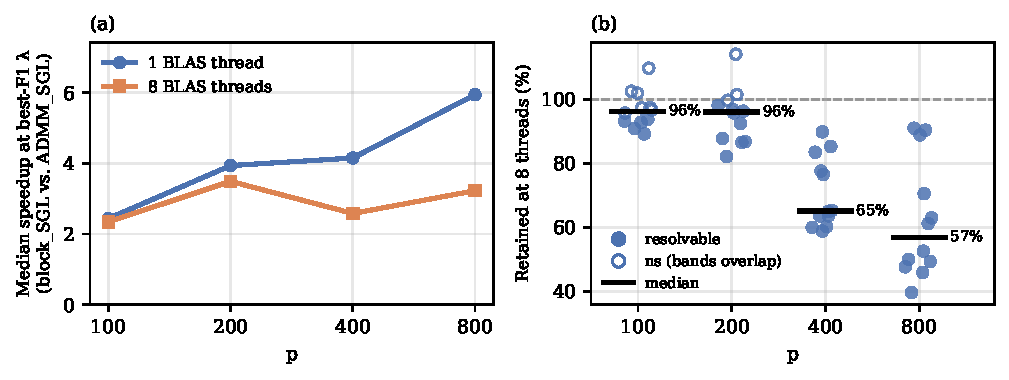
\includegraphics[width=0.85\textwidth]{fig1_rq1_threading.pdf}
\caption{(a) Median speedup at the best-F1 $\lambda$ with 1 and 8 BLAS
threads. (b) Speedup retained by the 8-thread baseline, per configuration;
hollow markers are not resolvable (overlapping trial bands). Seed 0; seeds
1--2 show the same pattern (text).}
\label{fig:threading}
\end{figure*}

\subsection{The over-fragmentation trap}
Table~\ref{tab:trap} pools all 384 configurations by detected block count.
Speedup rises monotonically with fragmentation, from $0.97\times$ to
$23.9\times$, while support F1 peaks at 0.75 in the 10--49 block range and
falls to 0.29 beyond 200 blocks (Fig.~\ref{fig:trap}). Reporting the fastest
configuration would claim a $24\times$ speedup on an estimate that is mostly
noise.

\begin{table}[t]
\centering
\caption{Speedup and estimation quality by detected block count
(1-thread run, 384 configurations).}
\label{tab:trap}
\begin{tabular}{rrrr}
\toprule
blocks & median speedup & median F1 & $n$ \\
\midrule
1 & $0.97\times$ & 0.152 & 50 \\
2--9 & $1.03\times$ & 0.490 & 21 \\
10--49 & $2.01\times$ & \textbf{0.750} & 77 \\
50--99 & $3.66\times$ & 0.734 & 58 \\
100--199 & $7.16\times$ & 0.654 & 60 \\
200+ & $\mathbf{23.93\times}$ & 0.286 & 118 \\
\bottomrule
\end{tabular}
\end{table}

\begin{figure}[t]
\centering
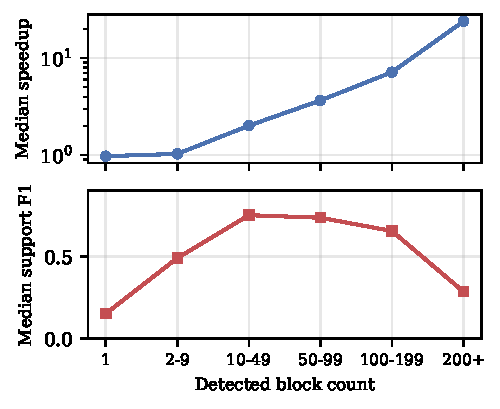
\includegraphics[width=0.82\columnwidth]{fig2_rq1_fragmentation_trap.pdf}
\caption{Speedup rises with fragmentation while estimation quality collapses.}
\label{fig:trap}
\end{figure}

\subsection{Where the time goes}
The cubic model predicts that the largest block dominates: at balanced
$p=800$, $n/p=10$, $\lambda=0.10$ the largest of 244 blocks (192 variables)
holds 99.6\% of the cubic work. Profiling contradicts this
(Table~\ref{tab:profile}): the largest single eigendecomposition is 1.4\% of
eigendecomposition time and under 1\% of wall-clock. The runtime is spread
over thousands of sub-millisecond eigendecompositions and Python per-block
glue (slicing, per-call solver setup, reassembly), which together account
for over 90\% of the time. The useful lever is therefore batching the
per-block work, not a faster eigensolver.

\begin{table}[t]
\centering
\caption{Profile of the decomposed solver (1 thread, median of 7).}
\label{tab:profile}
\begin{tabular}{lrr}
\toprule
 & imbalanced $p{=}200$ & balanced $p{=}800$ \\
 & $\lambda{=}0.15$ & $\lambda{=}0.10$ \\
\midrule
blocks (largest) & 58 (30) & 244 (192) \\
wall-clock & 24.1\,ms & 215\,ms \\
eigendecomposition & 31\% & 58\% \\
Python glue & 62\% & 35\% \\
component detection & 3\% & 4\% \\
eigh calls (mean) & 801 (0.01\,ms) & 2302 (0.05\,ms) \\
largest eigh, share & 0.9\% & 1.4\% \\
\bottomrule
\end{tabular}
\end{table}

\subsection{Why the true blocks merge}
Fig.~\ref{fig:oracle} compares the largest component's work share
$F_{\max}$ at the best-F1 $\lambda$ with the share the true block structure
would allow (oracle). For balanced and many\_tiny the truth leaves 80--97.5\%
of the work outside the largest block, yet the detected components leave
almost none (median $F_{\max}$ 99.9\%).

\begin{figure}[t]
\centering
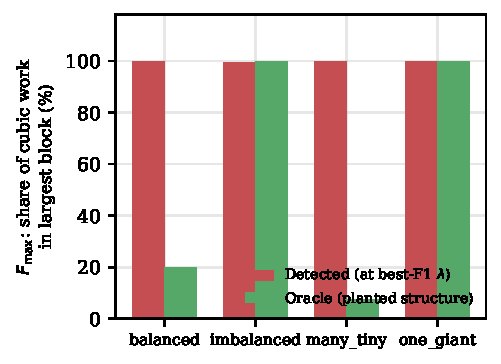
\includegraphics[width=0.82\columnwidth]{fig3_rq1_oracle_gap.pdf}
\caption{Largest-component work share at the best-F1 $\lambda$ (detected)
versus the true block structure (oracle), three seeds.}
\label{fig:oracle}
\end{figure}

This is not a failure of detection. We verified exactness of screening on
our instances: solving \eqref{eq:glasso} without decomposition (tol
$10^{-10}$) and taking components of the solution's support gives a
partition identical to thresholded-$S$ screening in 36 of 36 best-F1
configurations ($p\le400$). The giant component belongs to the graphical
lasso estimate itself.

The mechanism is connectivity. Counting above-threshold entries of $S$ that
join two different true blocks (72 best-F1 cells, three seeds), only a
median 3--4\% of entries cross true blocks in the balanced regime, e.g.\
33--42 of $\approx1900$ at $p=800$, $n/p=10$. That is enough to fuse all five
true blocks in every cell at $p\ge400$, and in the median cell at $p=200$. Overall, the largest component fuses at least
two true blocks in 68 of 72 cells. Support F1 barely registers 3\% spurious
entries, while parallelism collapses. Because screening is exact, any finer
partition, such as a higher threshold or a shrunk covariance, no longer
yields the graphical lasso solution: recovering this parallelism means
trading exactness for speed.

Thresholding $S$ and taking components is a percolation process, and
Fig.~\ref{fig:percolation} shows its cliff. At balanced $p=400$, $n/p=10$
the largest component holds essentially all the cubic work up to
$\lambda\approx0.14$ and drops to under 40\% by $\lambda=0.16$ (median of
three seeds). The best-F1 $\lambda$ (0.10) sits on the plateau, left of the
cliff: at the statistically useful operating point, the giant component has
not yet broken up. Near the cliff the structure is also unstable across
draws: at $\lambda=0.14$ the largest component holds 87\% and 55\% of the
work for two seeds, and 100\% for the third.

\begin{figure}[t]
\centering
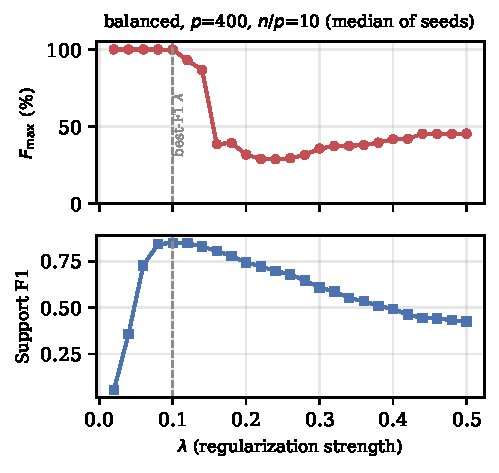
\includegraphics[width=0.82\columnwidth]{fig4_rq1_percolation.pdf}
\caption{Percolation cliff at balanced $p=400$, $n/p=10$ (median of three
seeds): largest-component work share $F_{\max}$ and support F1 against
$\lambda$. The best-F1 $\lambda$ lies on the plateau, before the giant
component breaks.}
\label{fig:percolation}
\end{figure}

\subsection{Batched execution on CPU and GPU}
Using the batched solver of Section~\ref{sec:batched}, on the
CPU batching alone gives $1.25$--$1.69\times$ over \texttt{block\_SGL} at
the best-F1 $\lambda$ ($p=200$--$800$, imbalanced and many\_tiny).

We report GPU performance as $S_{\mathrm{GPU}}=T_{\mathrm{CPU}}/T_{\mathrm{GPU}}$,
the batched CPU time (float64) over the batched GPU time, so $S_{\mathrm{GPU}}>1$
means the GPU is faster. On the GPU in double precision, our reference
configuration, the same batched code has $S_{\mathrm{GPU}}=0.10$--$0.79$
(i.e.\ $1.3$--$10\times$ \emph{slower}) at these sizes, and in a $\lambda$ scan
at $p=2000$ it first wins only at $s_{\max}\approx1950$
($1.07\times$). Transfers are at most 0.3\% of GPU time; the loss is
per-iteration launch overhead plus the reduced double-precision throughput of
a consumer GPU.

\textbf{Precision diagnostic.} To separate precision from batching, we
added a float32 GPU path and
pre-registered acceptance criteria before measuring it: all problems
converge at the unchanged tolerance; relative objective difference
$\le10^{-6}$; elementwise relative error $\le10^{-3}$ and no more than
$10\times$ the float64 solver's own distance to a high-accuracy solution;
support disagreement $\le0.1\%$ with no flips of clearly nonzero entries; and
F1 within 0.005. Float32 passed every criterion on four diagnostic points.
Its deviation from float64 ($3\times10^{-5}$--$1.4\times10^{-4}$ relative)
is 6--50$\times$ smaller than float64's own deviation from the high-accuracy
solution at the same stopping tolerance, and the objective agrees to within
$1.3\times10^{-8}$.

Across the full scan (Fig.~\ref{fig:crossover}), float32 moves the GPU
crossover from $s_{\max}\approx1950$ to $\approx650$, and peak GPU memory
roughly halves.

A float32 GPU compared with a float64 CPU is not a like-for-like comparison,
so we also timed a float32 CPU solver in the same session at every point.
Single precision does not help the CPU here: float32 NumPy is a median
$0.98\times$ the speed of float64 (range $0.62$--$1.32\times$) with the same
OpenBLAS eigensolver. In this session, for $s_{\max}\ge1000$ in the scan
the float32 GPU is $2.6$--$6.7\times$ faster than the float64 CPU and
$2.5$--$10.2\times$ faster than the float32 CPU; the upper end of the latter
comes from a point ($s_{\max}=1951$) where float32 was $1.5\times$
\emph{slower} than float64 on the CPU. At the two held-out anchors
($s_{\max}=2001$ and $3006$) the float32 GPU is $7.3\times$ and $9.6\times$
faster than the float64 CPU, and $6.9\times$ and $9.0\times$ faster like for
like (Table~\ref{tab:fp32}). Like for like, it overtakes the float32 CPU at
$s_{\max}\approx500$--$700$.

Float32 is not a free replacement on the GPU, however. In 13 of 36 scan
configurations, all with $s_{\max}\le112$, the float32 GPU solver fails to
converge within 1000 iterations, whereas float64 needs at most 329. The
float32 CPU solver, with the same stopping test, converges at every point,
so the failure is specific to the GPU single-precision path rather than to
single precision as such; we have not isolated its cause. Single precision on
the GPU is therefore viable exactly where the GPU wins, and float64 (or a
size-dependent precision policy) is needed for small blocks.

\begin{table}[t]
\centering
\caption{Float32 GPU speedup over the batched CPU solver, one session,
converged points only. Scan rows: $p=1200$ and $2000$; anchors: $p=2400$
and $3200$.}
\label{tab:fp32}
\begin{tabular}{lrr}
\toprule
$s_{\max}$ & vs.\ CPU float32 & vs.\ CPU float64 \\
\midrule
$<200$ & $0.08$--$0.26\times$ & $0.08$--$0.26\times$ \\
$200$--$640$ & $0.44$--$1.01\times$ & $0.40$--$1.16\times$ \\
$640$--$1000$ & $1.19$--$2.93\times$ & $1.24$--$3.38\times$ \\
$\ge1000$ & $\mathbf{2.45}$--$\mathbf{10.2\times}$ & $2.56$--$6.65\times$ \\
\midrule
anchor $2001$ & $6.87\times$ & $7.33\times$ \\
anchor $3006$ & $8.96\times$ & $9.62\times$ \\
\bottomrule
\end{tabular}
\end{table}

\begin{figure}[t]
\centering
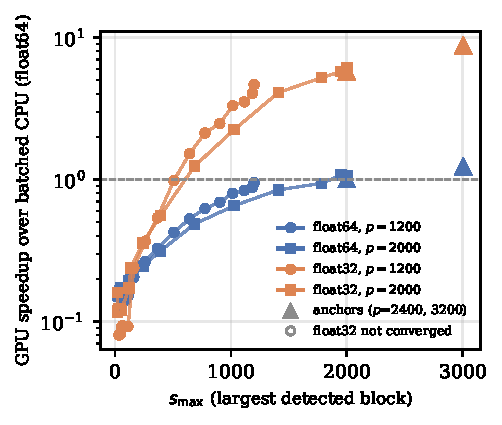
\includegraphics[width=0.82\columnwidth]{fig5_rq2_crossover.pdf}
\caption{GPU speedup over the batched CPU solver against the largest
block size, in float64 and float32 on the GPU (CPU baseline float64).
Hollow markers: float32 runs that did not converge.}
\label{fig:crossover}
\end{figure}

\subsection{GPU memory}
Peak GPU memory follows a quadratic model in $s_{\max}$ fitted on
$s_{\max}\le2000$ ($R^2=1.000$), which predicts two held-out anchors
($s_{\max}=2001$ and $3006$) within 0.2\% (Fig.~\ref{fig:vram}). On the 7.7\,GB visible to CUDA,
float64 reaches the limit only at $s_{\max}\approx8200$. Memory is not the
binding constraint in any regime we measured; float32 halves it.

\begin{figure}[t]
\centering
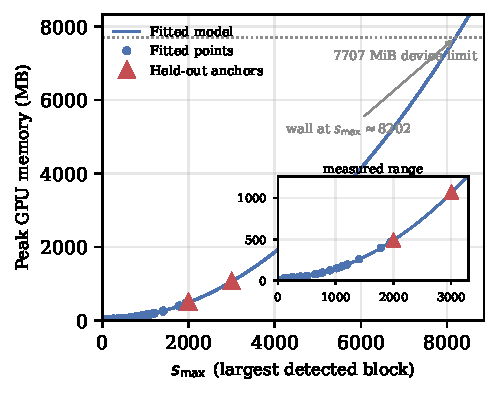
\includegraphics[width=0.82\columnwidth]{fig7_rq3_vram_model.pdf}
\caption{Peak GPU memory (float64) against the largest block size: quadratic
model fitted on $s_{\max}\le2000$ (inset: measured range) and two held-out
anchors, extrapolated to the 7707\,MiB visible to CUDA.}
\label{fig:vram}
\end{figure}

% =====================================================================
\section{Reproducibility lessons}
\label{sec:repro}
Two faults invalidated earlier versions of these datasets. Neither raised an
error.

\textbf{Thread-dependent random data.} GGLasso's sampler uses
\texttt{multivariate\_normal} with an SVD of $\Sigma$. Our block-diagonal
$\Sigma$ has repeated eigenvalues, so the singular vectors returned by
OpenBLAS, and hence the samples, depended on the BLAS thread count. The same
seed gave different data at 1 and 8 threads, and an earlier ``paired''
threading comparison agreed on detected structure in only 141 of 384
configurations. Sampling through the unique Cholesky factor makes the data
identical across thread counts to $10^{-12}$; a regression test now guards
this.

\textbf{Uncontrolled machine state.} An unrelated container occupying two
cores, together with an unrecorded power profile, slowed 8-thread CPU runs
by a median 16\% per iteration while leaving single-threaded runs
unaffected. CPU-only speedup ratios survived because both solvers slowed
together, but every GPU-versus-CPU ratio was inflated by about 30\%. Every run
now records CPU, BLAS library, power profile, load and running containers.

A clean reinstall from the published package lock reproduces the
structural results (detected blocks, objective values, F1) bit for bit on a
16-configuration check.

% =====================================================================
\section{What generalises}
The findings fall into two classes. The \emph{structural} results are
properties of the estimator and the data, not of our hardware: exactness of
screening, the fusion of true blocks by a few spurious cross-block entries,
the percolation cliff, and the opposition between fragmentation and
estimation quality. They are deterministic given the seed, identical across
BLAS thread counts, and would hold for any exact solver that uses component
screening, including other graphical lasso implementations. They bound
block parallelism for \emph{any} hardware: if the useful $\lambda$ leaves one
giant component, no parallel scheme over components can beat the time to
solve that component.

The \emph{performance} results are platform-dependent and should be read as
measurements of one CPU, one BLAS library and one consumer GPU: how much a
multithreaded baseline erodes the decomposition gain depends on how well the
BLAS parallelises one large eigendecomposition, and the GPU crossover depends
on per-launch overhead and the double-precision rate. We expect the
qualitative pattern (decomposition helps most at moderate $p$; a GPU helps
only on large blocks) to transfer, but the crossover block sizes will move.
A data-centre GPU with full-rate double precision should narrow the gap
between our float64 and float32 crossovers. To make these measurements
repeatable elsewhere, we release a one-command run package that reproduces
every experiment on another machine and records its environment.

% =====================================================================
\section{Limitations}
All measurements use one laptop; timings are machine-specific, and the
consumer GPU's double-precision rate is not representative of data-centre
GPUs. Data are synthetic, and the \emph{balanced} and \emph{many\_tiny}
regimes coincide at $p=100$.
CPU speedups and all structural results use three
independent instances; the GPU results use one (seed 0), so the GPU crossover
sizes carry instance-to-instance variation we did not measure. In four cells (three in seed 0, one in seed 2; all one\_giant at $p=800$)
the statistically best $\lambda$ lies below our timing grid
(Section~\ref{sec:speedup}); they are excluded from the reported medians. The float32 study covers one regime: every float32 measurement (scan,
anchors, diagnostic and CPU baseline) uses many\_tiny. The cause of GPU
float32 non-convergence on small blocks is not isolated. Timings compare against GGLasso's own
solvers; we do not benchmark QUIC or coordinate-descent implementations, and
F1 is computable only because the data are synthetic.

% =====================================================================
\section{Conclusion}
Exact component screening makes the graphical lasso look embarrassingly
parallel, but at statistically useful regularisation little of that
parallelism survives. The estimator fuses the true blocks through a handful
of spurious entries, the work that remains is dominated by per-block overhead
rather than arithmetic, and a multithreaded CPU baseline recovers much of the
apparent gain. Batching recovers $1.2$--$1.7\times$ on the CPU. On a
consumer GPU, precision rather than batching decides the outcome: in single
precision the GPU is $2.5$--$10\times$ faster than a like-for-like CPU on
blocks of 1000 or more variables (Table~\ref{tab:fp32}), while small blocks need double precision to converge on the
GPU. The binding constraint on block parallelism is the
estimator's structure, not the hardware.

\bibliographystyle{IEEEtran}
\bibliography{refs}

\end{document}
